\documentclass[10pt]{beamer}

\usepackage[utf8]{inputenc}
\usepackage[czech]{babel}
\usepackage{amsmath,amsthm,amssymb,hyperref}
\usepackage{graphicx,color,tabularx,float,caption,subcaption,nicefrac}

\mode<presentation>{
	\usetheme{Malmoe}
	\usecolortheme{crane}
	\setbeamertemplate{blocks}[default]
	
	\setbeamertemplate{section in toc}{\inserttocsectionnumber.~\inserttocsection}
	\setbeamertemplate{subsection in toc}{\hspace{1.2em}{\scriptsize\raise0.25pt\hbox{\color[rgb]{0.99,0.73,0.02}$\blacksquare$}}~\inserttocsubsection\par}
	
	\setbeamertemplate{itemize item}{\scriptsize\raise0.5pt\hbox{\color[rgb]{0.99,0.73,0.02}$\blacksquare$}}
	\setbeamertemplate{itemize subitem}{\tiny\raise0.5pt\hbox{\color[rgb]{0.99,0.73,0.02}$\blacksquare$}}
	\setbeamertemplate{itemize subsubitem}{\tiny\raise0.5pt\hbox{\color[rgb]{0.99,0.73,0.02}$\blacksquare$}}
	\setbeamertemplate{enumerate item}{\insertenumlabel.}
	\setbeamertemplate{enumerate subitem}{\insertenumlabel.\insertsubenumlabel}
	\setbeamertemplate{enumerate subsubitem}{\insertenumlabel.\insertsubenumlabel.\insertsubsubenumlabel}
	\setbeamertemplate{navigation symbols}{}
	\setbeamertemplate{headline}{
		\begin{beamercolorbox}[ht=10pt]{section in head/foot}
			\vskip2pt\insertsectionnavigationhorizontal{\paperwidth}{}{\hskip0pt plus1filll}\vskip2pt
		\end{beamercolorbox}
		\begin{beamercolorbox}[ht=10pt]{subsection in head/foot}
			\vskip2pt\insertsubsectionnavigationhorizontal{\paperwidth}{}{\hskip0pt plus1filll}\vskip2pt
		\end{beamercolorbox}
	}
}

\renewcommand{\P}{\mathsf{P}}
\newcommand{\NP}{\mathsf{NP}}
\newcommand{\coNP}{\mathsf{co}\textnormal{-}\mathsf{NP}}
\newcommand{\RP}{\mathsf{RP}}
\newcommand{\coRP}{\mathsf{co}\textnormal{-}\mathsf{RP}}
\newcommand{\BPP}{\mathsf{BPP}}
\newcommand{\BQP}{\mathsf{BQP}}
\newcommand{\ZPP}{\mathsf{ZPP}}
\newcommand{\DTime}{\mathsf{DTime}}
\newcommand{\NTime}{\mathsf{NTime}}
\newcommand{\DSpace}{\mathsf{DSpace}}
\newcommand{\NSpace}{\mathsf{NSpace}}
\newcommand{\BPTime}{\mathsf{BPTime}}
\newcommand{\RTime}{\mathsf{RTime}}
\newcommand{\ZPTime}{\mathsf{ZPTime}}
\newcommand{\atam}{\mathsf{aTAM}}
\newcommand{\ktam}{\mathsf{kTAM}}
\newcommand{\myatam}{\mathsf{DaTAM}}
\renewcommand{\iff}{\Leftrightarrow}
\newcommand{\then}{\Rightarrow}
\newcommand{\R}{\mathbb{R}}
\newcommand{\Z}{\mathbb{Z}}
\newcommand{\N}{\mathbb{N}}
\newcommand{\prob}{\mathbb{P}}
\newcommand{\indicator}{\mathds{1}}
\newcommand{\powerset}[1]{\mathcal{P} ( #1 )}
\newcommand{\adob}[2]{#1 , \ldots , #2}
\let\epsilon\varepsilon
\let\phi\varphi

\theoremstyle{definition}
\newtheorem{defn}{Definice}
\newtheorem{tvr}{Tvrzení}
% \newtheorem{lemma}{Lemma}   % je definováno defaultně
\newtheorem{teze}[tvr]{Téze}
\newtheorem{domn}[tvr]{Domněnka}
\newtheorem{dusl}[tvr]{Důsledek}
\newtheorem{castDuk}{Důkaz.}   % pro část důkazu, bez čtverečku
\newtheorem{prikl}{Příklad}
\newtheorem{alg}[tvr]{Algoritmus}

\theoremstyle{remark} 
\newtheorem{pozn}{Poznámka}

% ======================================================================
%
%    S T A R T
%
% ======================================================================

\title{Modely sebeskládajících DNA nanostruktur}
\institute
{
	Fakulta jaderná a fyzikálně inženýrská\\
	Matematická informatika
}
\author{Vypracoval: Jakub Klemsa\\
	~\\
	Školitel: Ing. Štěpán Starosta, Ph.D.}
\date{19. června 2014}

\begin{document}

\begin{frame}
	\titlepage
\end{frame}

\begin{frame}
	\tableofcontents
\end{frame}

%~ \begin{frame}{Table of Contents}   % průběžný obsahy
%~ \tableofcontents[currentsection,currentsubsection,hideothersubsections,sectionstyle=show/shaded,]
%~ \end{frame}

\section{Úvod}
\begin{frame}
\frametitle{Úvod}
	První experiment s DNA -- L. Adleman, 1994, \cite{adleman94}
	\begin{itemize}
		\item hledání Hamiltonovské cesty (HC) orientovaným grafem
		%~ \item HC projde každý vrchol grafu právě jednou, počáteční a cílový vrchol jsou zadány
		\item rozhodovací problém existence HC je $\NP$-úplný
	\end{itemize}
\end{frame}

\begin{frame}
\frametitle{Úvod}
	Výhody
	\begin{itemize}
		\item paralelizmus -- ve zkumavce až $10^{18}$ \uv{větších} molekul
		\item energetická efektivita (Adleman \cite{adleman94})
	\end{itemize}
	\pause
	Nevýhody
	\begin{itemize}
		\item na $10^{18}$ operací stačí hrubá síla (řádově dny na clusteru s tisíci jader)
		\item pravděpodobnostní povaha
		\item chybovost
	\end{itemize}
	\pause
	Pole studia
	\begin{itemize}
		\item kinetika reakcí
		\item {\bf abstraktní modely pohledem matematické informatiky}
	\end{itemize}
\end{frame}

\section{DNA vs. Chomského hierarchie}
\subsection{Regulární jazyky}
\begin{frame}
\frametitle{Souvislost s Chomského hierarchií}
	Lineární vlákna $\leftrightarrow$ regulární jazyky (Winfree \cite{winfree_phd})
	\begin{figure}[h]
	\begin{center}
		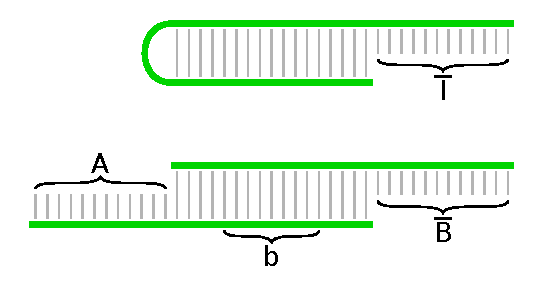
\includegraphics[width=0.502\textwidth]{../figures/strand_types/linear.pdf} % {šířka v mm}/370 je to původně
		\caption{Vlákno pro iniciální symbol $I$ a vlákno pro pravidlo $A\rightarrow bB$.}
	\end{center}
	\end{figure}
	$\overline{B}$ značí Watson-Crick komplementární sekvenci k $B$ ($A \leftrightarrow T$, $C \leftrightarrow G$)
\end{frame}

\subsection{Bezkontextové jazyky}
\begin{frame}
\frametitle{Souvislost s Chomského hierarchií}
	Stromové struktury $\leftrightarrow$ bezkontextové jazyky (Winfree \cite{winfree_phd})
	\begin{figure}[h]
	\begin{center}
		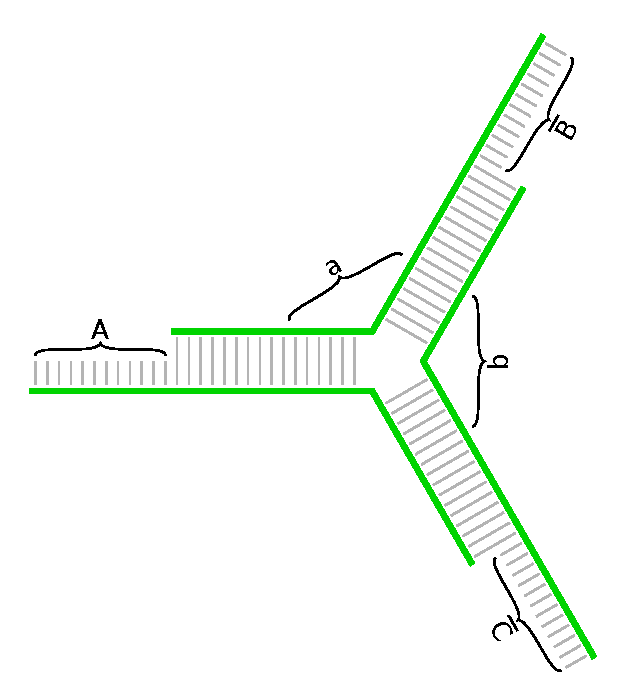
\includegraphics[width=0.502\textwidth]{../figures/strand_types/dendrimer.pdf} % {šířka v mm}/370 je to původně
		\caption{Struktura odpovídající pravidlu $A\rightarrow aBbC$.}
	\end{center}
	\end{figure}
\end{frame}

\subsection{Turingova univerzalita}
\begin{frame}
\frametitle{Souvislost s Chomského hierarchií}
	Dvojkřížené molekuly $\leftrightarrow$ Turingův stroj (TS) (Winfree \cite{winfree_phd})
	\begin{figure}[h]
	\begin{center}
		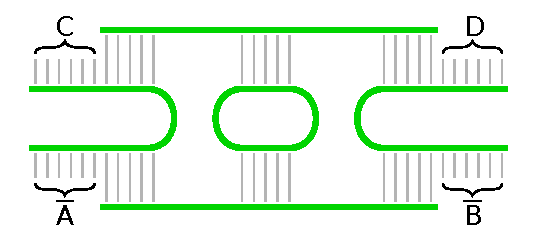
\includegraphics[width=0.502\textwidth]{../figures/strand_types/double_crossover.pdf} % {šířka v mm}/370 je to původně
		\caption{Dvojkřížená molekula, velmi stabilní (Seeman, Fu \cite{seeman93}).}
	\end{center}
	\end{figure}
\end{frame}

\section{Modely založené na Wangovo dláždění}
\subsection{Wangovo dláždění}
\begin{frame}
\frametitle{Wangovo dláždění}
	Čtvercové dláždění roviny (její části), kde
	\begin{itemize}
		\item dlaždice mají na hranách barvu z konečné množiny barev (lepidel)
		\item jsou orientované (zakázáno rotovat nebo překlápět)
		\item sousedit smí pouze dlaždice se stejnou barvou na společné hraně
	\end{itemize}
	\begin{figure}[h]
	\begin{center}
		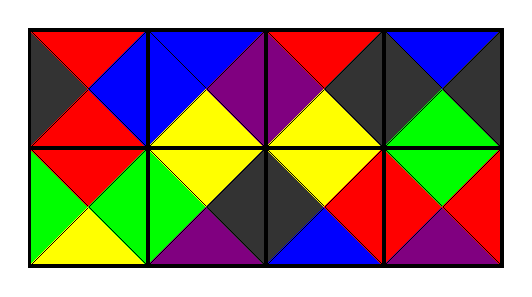
\includegraphics[width=0.4\textwidth]{../figures/wang_tiling/wang_tiling.pdf} % {šířka v mm}/370 je to původně
		\caption{Wangovo dláždění.}
	\end{center}
	\end{figure}
\end{frame}

\subsection{$\atam$}
\begin{frame}
\frametitle{$\atam$}
	Rothemund, Winfree rozšířili definici
	\begin{itemize}
		\item každé lepidlo má přidružené přirozené číslo -- síla lepidla
		\item existuje prázdné lepidlo se silou 0, které smí sousedit se všemi
		\item dláždění se utváří
		\begin{itemize}
			\item z iniciální dlaždice
			\item po jedné dlaždici
			\item součet právě připojených lepidel musí být větší nebo roven zadané hodnotě (tzv. {\em teplota}, ozn. $\tau$)
		\end{itemize}
	\end{itemize}
\end{frame}

\subsection{Studované složitosti}
\begin{frame}
\frametitle{Studované složitosti I}
	Biostep complexity $Bs(n)$
	\begin{itemize}
		\item počet laboratorních procedur (popsané v Adleman \cite{adleman95biostep}, Winfree \cite{winfree_phd})
		\item jedna trvá až desítky minut
		\item za proveditelné budeme uvažovat pouze $Bs(n) \in O(1)$
	\end{itemize}
	Binding complexity $Bnd(n)$
	\begin{itemize}
		\item počet vazeb v koncovém dláždění
		\item v nedeterministickém případě uvažujeme nejmenší přijímací
		\item v pravděpodobnostním případě uvažujeme střední hodnotu
		\item kvůli rostoucí psti chyby -- proveditelné $Bnd(n)$ polynomiální
	\end{itemize}
\end{frame}

\begin{frame}
\frametitle{Studované složitosti II}
	Tile complexity $Ti(n)$
	\begin{itemize}
		\item počet různých dlaždic
		\item potřeba je syntetizovat -- proveditelné $Ti(n)$ polynomiální
	\end{itemize}
	Glue complexity $Gl(n)$
	\begin{itemize}
		\item počet různých lepidel -- sekvencí
		\item příliš dlouhé se mohou vázat chybně -- proveditelné $Gl(n)$ polynomiální
	\end{itemize}
	\pause
	\begin{lemma}
		\begin{enumerate}
			\item $Ti(n) \leq Gl^4(n)$,
			\item $Gl(n) \leq 4\,Ti(n)$.
		\end{enumerate}
	\end{lemma}
\end{frame}

\subsection{Výpočetní síla $\atam$u}
\begin{frame}
\frametitle{Výpočetní síla $\atam$u}
	$\atam$ je Turingovsky univerzální (TU)
	\begin{itemize}
		\item ve 2D při teplotě $\tau=2$, Winfree \cite{winfree_phd}
		\item ve 3D při teplotě $\tau=1$, Cook \cite{cook_temp1}
	\end{itemize}
	Neví se ve 2D při teplotě $\tau=1$
	\begin{itemize}
		\item existují modifikace $\atam$u, které jsou TU
	\end{itemize}
	Důkaz TU ve 2D při teplotě $\tau=2$ -- převod na celulární automat
	\begin{itemize}
		\item neříká nic o spotřebě zdrojů
	\end{itemize}
\end{frame}

\subsection{Jiný důkaz TU}
\begin{frame}
\frametitle{Důkaz TU ve 2D při $\tau=2$}
	\begin{itemize}
		\item přímočarý
		\item včetně odhadů studovaných složitostí v závislosti na čase a prostoru spotřebovaným simulovaným TS
		\item v práci str. 15-16
	\end{itemize}
\end{frame}

\subsection{Meze studovaných složitostí}
\begin{frame}
\frametitle{Meze studovaných složitostí}
	\begin{lemma}
		Studované složitosti v tomto systému jsou omezené:
		\begin{description}
			\item[Biostep.] $Bs(n) \in O(1)$.
			\item[Binding.] $Bnd(n) \in O\bigl(s(n)\cdot t(n)\bigr)$, kde $t(n)$ je čas a $s(n)$ prostor spotřebovaný simulovaným TS.
			\item[Tile.] $Ti(n) \in O(n)$.
			\item[Glue.] $Gl(n) \in O(n)$.
		\end{description}
	\end{lemma}
\end{frame}

\subsection{Důsledky}
\begin{frame}
\frametitle{Proveditelnost $\BPP$ ve 2D při $\tau=2$}
	$\BPP$ je třída jazyků rozhodnutelných pravděpodobnostním Turingovým strojem (PTS) v~polynomiálním čase, považuje se za proveditelnou\\
	~\\
	Z~předchozího lemmatu plyne:
	\begin{dusl}
		$\BPP$ je proveditelná v modelu $\atam$ ve 2D při $\tau=2$.
	\end{dusl}
	\begin{pozn}
		$\P$, $\ZPP$, $\RP$, $\coRP \subseteq \BPP$.
	\end{pozn}
\end{frame}

\section{Návrh řešení $\NP$ problémů}
\subsection{Přizpůsobení modelu $\NP$}
\begin{frame}
\frametitle{Přizpůsobení $\atam$u řešení $\NP$ problémů}
	Odvozen z Winfreeho ukázky řešení problému Hamiltonovské cesty -- avšak srozumitelnější
	\begin{itemize}
		\item $\tau=2$
		\item $5$ dalších typů dlaždic včetně daných sil lepidel
		\item pevně nastavená počáteční $t_0$
	\end{itemize}
	\begin{pozn}
		Tento model lze snadno simulovat klasickým $\atam$em.
	\end{pozn}
\end{frame}

\begin{frame}
	\begin{figure}[H]
	\begin{center}
		\begin{subfigure}[b]{0.33\textwidth}
			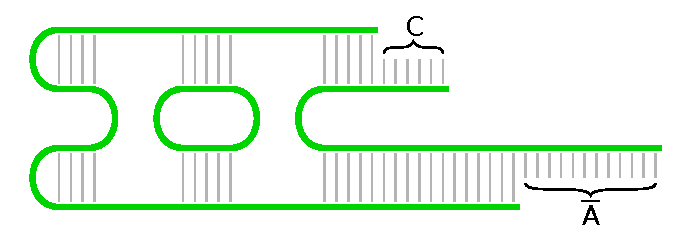
\includegraphics[width=\textwidth]{../figures/tile_model/DNA_struct.pdf} % 115mm
			\caption{Rohová molekula}
		\end{subfigure}
		\begin{subfigure}[b]{0.65\textwidth}
			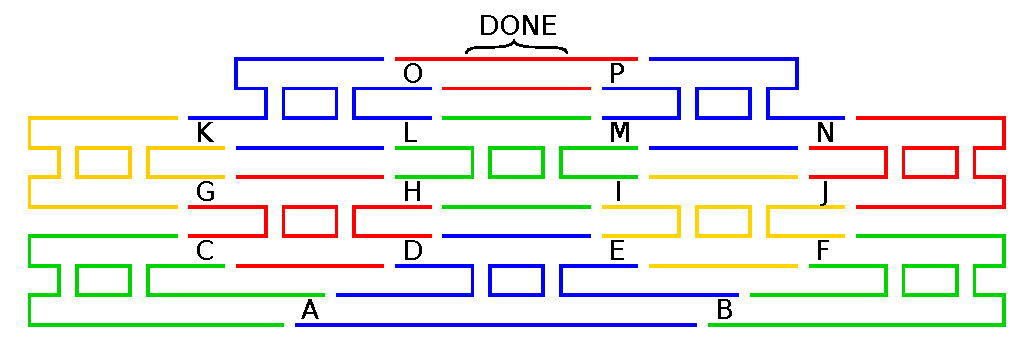
\includegraphics[width=\textwidth]{../figures/tile_model/DNA_assembly.pdf} % 175mm
			\caption{Schéma sebeskladu}
		\end{subfigure}
		\begin{subfigure}[b]{0.25\textwidth}
			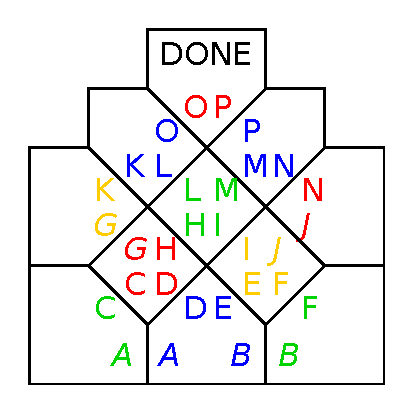
\includegraphics[width=\textwidth]{../figures/tile_model/abstract_model.pdf} % 70mm
			\caption{Model}
		\end{subfigure}
		\caption{Evoluce modelu od molekul k dlaždicím. Zde lepidla {\sf A}, {\sf B}, {\sf G} a {\sf J} mají sílu $2$, všechna ostatní mají sílu $1$.}
		\label{fig:evolution}
	\end{center}
	\end{figure}
\end{frame}

\subsection{Problém $k$-kliky}
\begin{frame}
\frametitle{Problém $k$-kliky}
	$\NP$-úplný problém, $Bnd \sim \nicefrac{5}{4}k^2$, $Ti \sim 2k^2e + 3kn$, $Gl \sim kn$.
	\begin{figure}[h]
	\begin{center}
		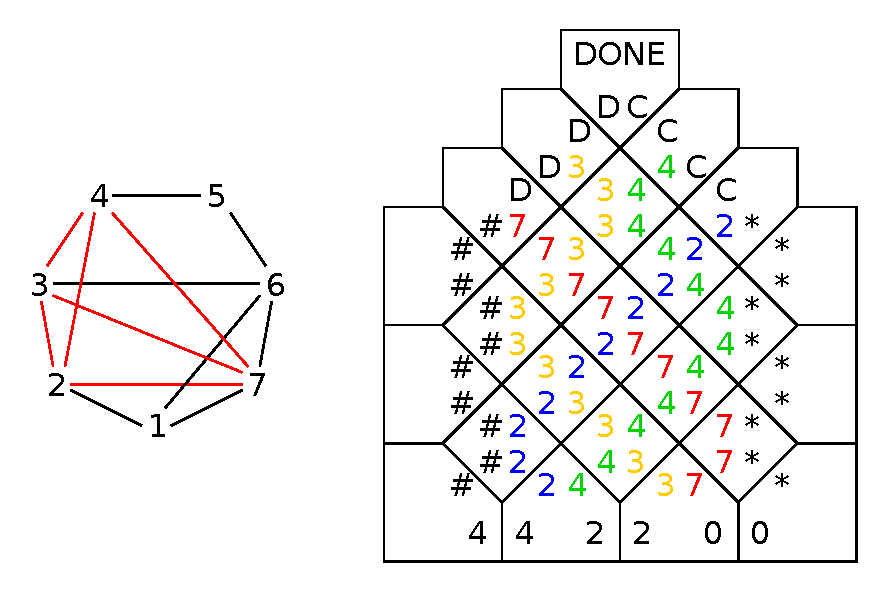
\includegraphics[scale=0.6]{../figures/k-clique/k-clique.pdf}
		\caption{Nalezení $k$-kliky. Řazení barev je dáno jejich vlnovou délkou.}
	\end{center}
	\end{figure}
\end{frame}

\subsection{Počítačová simulace}
\begin{frame}
\frametitle{Simulace v $\tt xgrow$}
	$\tt xgrow$ je open-source simulátor jak kinetických tak abstraktních modelů.
	\begin{itemize}
		\item skriptem (na CD) k zadanému grafu generuji potřebné dlaždice
		\item se zapnutím kinetiky není jednoduché dosáhnout bezchybného dláždění
	\end{itemize}
\end{frame}

\subsection{Další vyřešené problémy}
\begin{frame}
\frametitle{Další vyřešené problémy}
	$3$-obarvení grafu
	\begin{itemize}
		\item $\NP$-úplný problém
	\end{itemize}
	Grafový izomorfizmus
	\begin{itemize}
		\item domnívá se, že není $\NP$-úplný
	\end{itemize}
\end{frame}

\section*{Reference}
\begin{frame}[allowframebreaks=0.95]
\frametitle{Reference}
	\bibliography{../biblio}{}
	\bibliographystyle{plain}
\end{frame}

\end{document}